


%-----------------------------------------------------------------------------
% Intro
%-----------------------------------------------------------------------------
\section{Atmospheric Neutrino Fit Methods}
\label{sec:methods}

The main objective of the atmospheric neutrino fit is to estimate a set of
systematic error parameters related to the fiTQun reconstruction performance,
which we denote as \ldsk.  The \ldsk parameters should encode the differences 
we expect to observe between running fiTQun on SK data and MC simulation.
Since these systematic differences arise in principle from fundamental mis-modeling of SK detector properties,
we refer them as SK ``detector uncertainties'' and we assume that the differences we observe
between the atmospheric data and atmospheric MC are representative of the differences between the
T2K data and T2K MC. 

To estimate the values of the SK detector systematics parameters, we compare
the MC predictions with various \ldsk parameters applied to the SK atmospheric
neutrino data. Formally, we wish to maximize (or sample from, in the context of
MCMC) the likelihood defined by:

\begin{equation}
  \label{eq:likelihood}
  \mathcal{L}(\mathbf{a},\mathbf{x_{atm}},\dsk|\mathbf{M_{SK}}) =
  P(\mathbf{M_{Atm-SK}}|\mathbf{a},\mathbf{x_{atm}},\dsk) \ast \pi(\mathbf{a})
  \ast \pi(\mathbf{x_{atm}}) \ast \pi(\dsk)
\end{equation}

In this equation, $\mathbf{a}$ are the atmospheric neutrino flux parameters,
$\mathbf{x_{atm}}$ are the atmospheric neutrino cross section parameters, and
$\mathbf{M_{Atm-Sk}}$ is the observed SK atmospheric neutrino data. This
equation was obtained through general considerations of the T2K oscillation fit
strategy as described in Section 2 of TN-186~\cite{tn186}.


%-----------------------------------------------------------------------------
% Fit Parameters
%-----------------------------------------------------------------------------
\subsection{Detector Systematic Uncertainty Parameterization}
\label{subsec:betapar}

There is no unique choice of detector systematic uncertainty parameters \ldsk.
The detector error parameterization has changed several times to best suit the
needs of each analysis. For this analysis, we use a parameterization
similar to that of TN-186 in which we directly modify the cut variables.  The
cut variables we wish to modify are the fiTQun reconstructed variables that are
used to define the topological cuts for the T2K \nue and \numu event
selections.  There are four such variables in total, and they are listed
in Table~\ref{tab:fqvars}.

For each event, we assign the $m$-th fiTQun cut variable $L_{m}$ a parameter
$\beta^{0}$ and a parameter $\beta^{1}$ that modify its value in the following
way:
%
\begin{equation}
  \label{eq:fqparmod}
  L_{m}' = \beta^{1} L_{m} + \beta^{0}
\end{equation}
%
In this parameterization, $\beta^{0}$ is a ``bias'' parameter that shifts the
entire $L_{m}$ distribution.  This parameter is used in the same way as the
$\beta$ parameters in previous SK atmospheric fits (see Equation 16 in TN-186).
The $\beta^{1}$, on the other hand, is a ``smearing'' parameter that adjusts
the $L_{m}$ distribution to be wider (for $\beta^{1} > 1$) or narrower (for
$\beta^{1} < 1$).  This multiplicative scaling parameter is introduced to
provide additional flexibility to fit for data/MC differences.  This especially
important in this analysis, since we will be fitting to the entire
distribution shape (see Section~\ref{subsec:parlike}).

\begin{table}
  \centering
  \begin{tabular}{c | c}
    \hline\hline
    Cut Variable $m$ & Cut Variable  Name \\
    \hline
    0 & fiTQun $e/\mu$ PID \\
    1 & fiTQun $e/\pi^{0}$ PID \\
    2 & fiTQun $\mu/\pi$ PID \\
    3 & fiTQun Ring-Counting Parameter \\
    \hline\hline
  \end{tabular}
  \caption{List of fiTQun cut variables include in this fit.  More details on
  how these variables are defined can be found in TN-319.}
  \label{tab:fqvars}
\end{table}

The impetus behind this parameterization comes from the observation that the
mis-modeling of fundamental parameters in the MC most prominently manifests
itself as shifts in the distributions of fiTQun reconstructed variables. This
can be seen, for example, in the stopping cosmic muon data, where the muon and
decay electrons exhibit a shift in the fiTQun electron/muon particle
identification (PID) parameter.  Furthermore,
significant shifts in the distributions of fiTQun variables are seen in regions
of the detector near the ID wall.  Since we wish to estimate the systematics in
these regions, it makes sense to directly fit for these shifts when comparing
MC to data. 

%\begin{figure}[hb]
%  \begin{center}
%    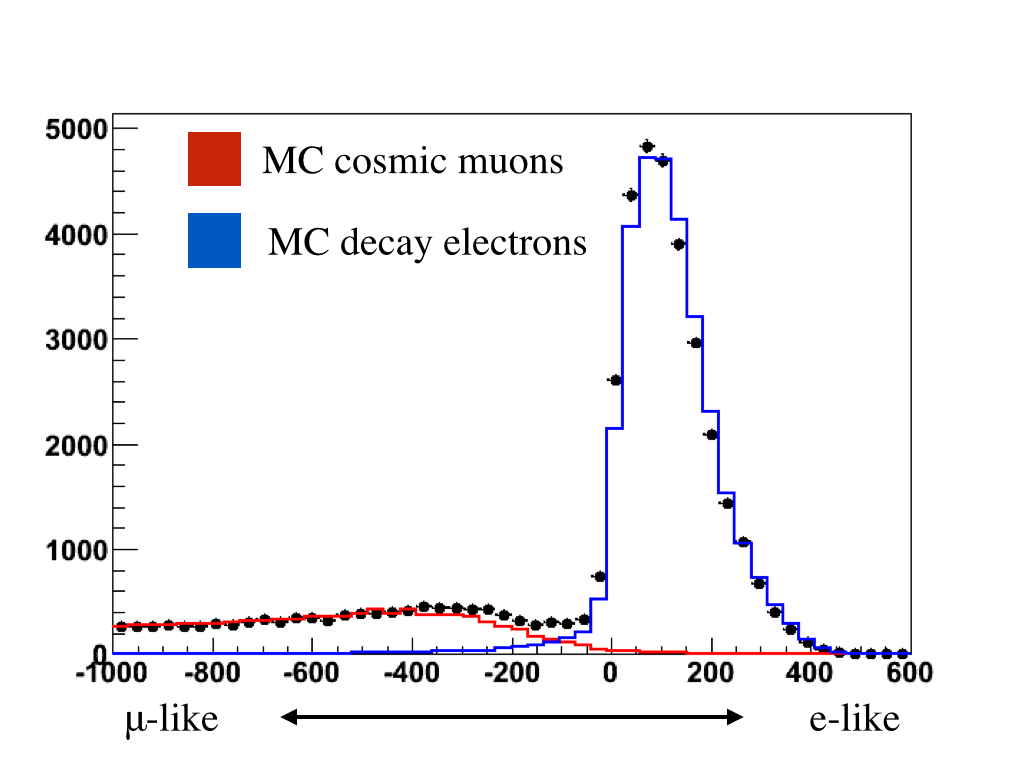
\includegraphics[width=0.6\textwidth]{cosmic_shift}
%  \end{center}
%  \caption{Distributions of the fiTQun $e/\mu$ PID parameter for MC stopping
%  cosmic muons (red) and the associated decay electrons (blue). Black points
%  show the observed data normalized to the MC\@. A shift in the distributions
%  between data and MC can be seen in both samples.}
%  \label{fig:shift}
%\end{figure}

The parameterization of detector uncertainties was chosen without detailed
knowledge of the actual data/MC discrepancies in the atmospheric data.  This
helps to ensure that the parameterization is not tuned to specific
discrepancies in the atmospheric data, which may arise from statistical
fluctuations or other sources besides the mis-modeling of detector parameters
that we are trying to measure.  



%-----------------------------------------------------------------------------
% Flux and Xsec Parameters
%-----------------------------------------------------------------------------
\subsection{Atmospheric Flux and Cross Section Parameterization}
\label{subsec:alphapar}

One difficulty in using atmospheric neutrino data to constrain SK detector
systematics is that the true distributions of the neutrino energy spectrum, the
flavor composition, and the interaction modes are not known precisely.  This is
due to the fact that there are significant uncertainties in the flux and cross
sections for atmospheric neutrino events.  Ideally, we wish to separate the
contributions of the flux and cross section uncertainties from the detector
systematic uncertainties, so that we may propagate only the components that
directly affect the T2K analyses. 

In principle, the cross section uncertainties are also shared between the
atmospheric and T2K analyses, so these parameters should be fit jointly with
the T2K data. Indeed, for future analyses, it may be preferable to use the T2K
cross section parameterization, which would allow these parameters to be
jointly estimated using both T2K and atmospheric neutrino data. Such a unified
approach is the subject of ongoing study by the T2K-SK group. For this
particular analysis, however, we adopt the strategy from previous atmospheric fits of
simultaneously fitting the atmospheric flux, cross section, and detector
systematics parameters to the atmospheric data, and then propagating only the
detector uncertainties to the T2K analysis. 

\begin{figure}[h]
  \begin{center}
    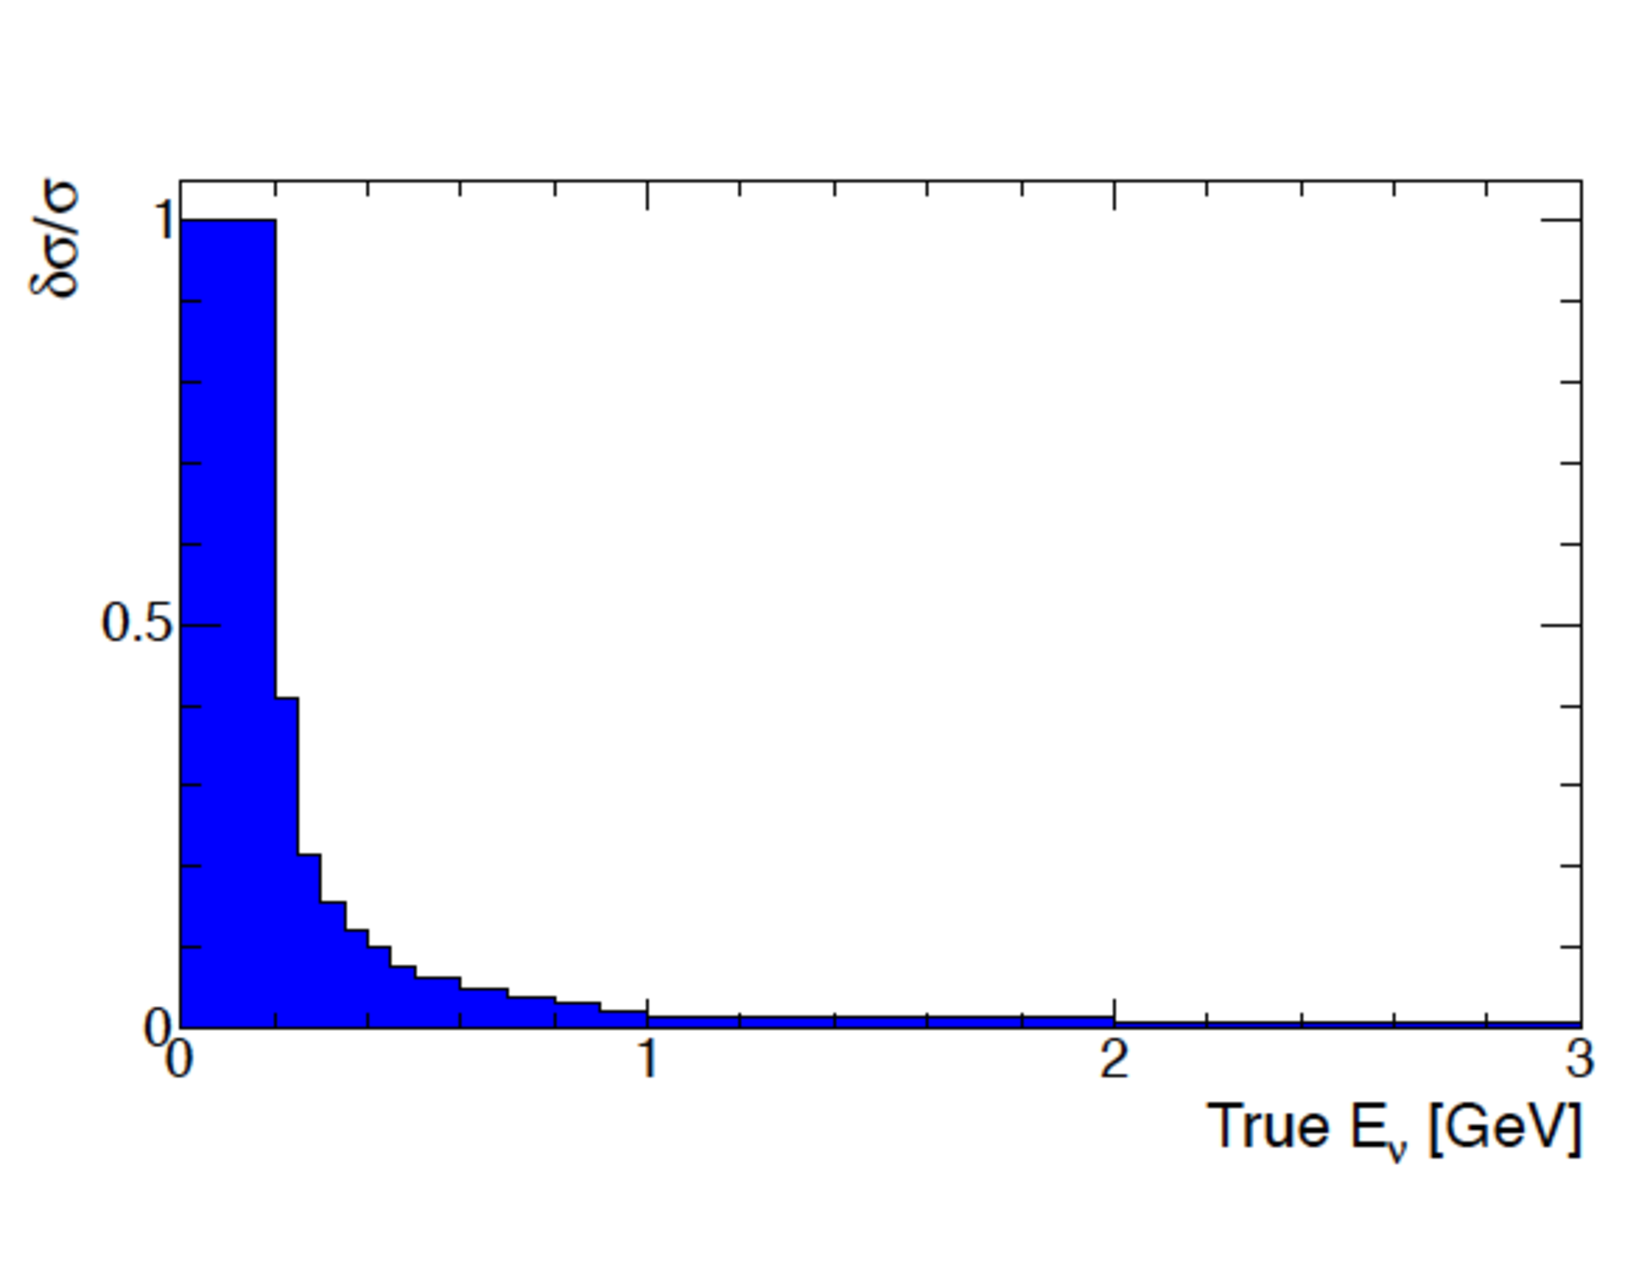
\includegraphics[width=0.5\textwidth]{tn186EnuXsec}
  \end{center}
  \caption{Dependence of the CCQE cross section uncertainty $\alpha_{CCQE}$ on
  the true neutrino energy.}
  \label{fig:alphaccqe}
\end{figure}

The parameterization of the atmospheric flux and cross section uncertainties in
this analysis is identical to that of TN-186~\cite{tn186}, which was in turn taken from
TN-157~\cite{tn157}, TN-159~\cite{tn159}, and TN-034~\cite{tn034}. The list of
flux and cross section parameters are shown in Table~\ref{tab:alpha}.  Each of
these 19 parameters are applied to the MC as a multiplicative factor that
affects only the events of the given ``Event Class'' in Table~\ref{tab:alpha}.

\begin{table}
  \centering
  \begin{tabular}{c c | c | c | c }
    \hline\hline
    n & Event Class & Parameter & Type & Prior Uncertainty $(\sigma_{\alpha})$ \\
    \hline 
    1 & $E_{\nu} <$ 1 GeV & $\alpha_{NormLowE}$ & Flux normalization & 0.25 \\
    1 & $E_{\nu} >$ 1 GeV & $\alpha_{NormHighE}$ & Flux normalization & 0.15 \\
    2 & CCQE & $\alpha_{CCQE}$ & Cross section & Figure~\ref{fig:alphaccqe} \\
    3 & CCnQE & $\alpha_{CCnQE}$ & Cross section & 0.20 \\
    4 & $\nu_{\mu}$ & $\alpha_{\nu_{mu}/\nu_{e}}$ & Cross section ratio & 0.05 \\
    5 & NC & $\alpha_{NC}$ & Cross section & 0.20 \\
    \hline\hline
  \end{tabular}
  \caption{Atmospheric flux and cross section parameters.  These parameter
  definitions are identical to those of T2K TN-186 Table 6. The event class is
  determined by cuts on the MC truth information.}
  \label{tab:alpha}
\end{table}




%-----------------------------------------------------------------------------
% MC Components
%-----------------------------------------------------------------------------
\subsection{MC Component Definitions}
\label{subsec:components}

The detector uncertainty parameters outlined in Section~\ref{subsec:betapar}
should be fit independently for different event topologies. The idea here is to
allow, for example, the events with a single muon ring to have shifts in the
reconstructed fiTQun quantities that are independent of the events with a
single electron ring.  To facilitate this, the MC is broken down into various
``components'', with each component containing a different visible event
topology that in principal could exhibit a different shift between the data and
simulation.  When defining the MC components, a balance must be struck between
accounting for many different topologies and having enough data statistics to
provide a constraint on it's distribution shapes.  The component definitions
chosen for this analysis are shown in Table~\ref{tab:components}.  These
components are defined purely in terms of their visible rings (as opposed to
the underlying interaction mode or particle type) since fiTQun is directly
sensitive to this information.  The visible rings are counted by iterating
through the simulated particles that exit the nucleus and identifying those
that are above Cherenkov threshold.

\begin{table}
  \centering
  \begin{tabular}{c | c | l }
    \hline\hline
    MC Component $k$ & Name & Definition (from MC truth) \\
    \hline
    0 & Single Electron & Single visible electron ring \\
    1 & Single Muon & Single visible muon ring  \\
    2 & Electron-like + Other & Visible electron ring with other visible rings  \\
    3 & Muon-like + Other & Visible muon ring with other visible rings  \\
    4 & Single $\pi^{0}$ & Single visible $\pi^{0}$  \\
    5 & Single Hadron &Single visible proton or pion  \\
    \hline\hline
  \end{tabular}
  \caption{Definitions of the MC components that are used in the atmospheric
  fit.  Each component is defined based on the true visible topology. Each of these
  components receives a separate set of the $\beta$ parameters described in
  Section~\ref{subsec:betapar}. }
  \label{tab:components}
\end{table}



%-----------------------------------------------------------------------------
% Detector Regions
%-----------------------------------------------------------------------------
\subsection{Detector Region Definitions}
\label{subsec:DR}

To accomplish the goal of estimating detector systematics in various SK
detector regions, we further separate the MC events by their location and
orientation in the SK detector volume.  We define a particular event's location
and orientation in terms of two variables: \wall and \towall.  Here \wall
refers to the minimum distance between the particle vertex and the ID wall, and
\towall refers to the distance along the reconstructed particle track to the ID
wall.  The definitions are sketched out in Figure~\ref{fig:fvdiag}.

\begin{figure}[h]
  \begin{center}
    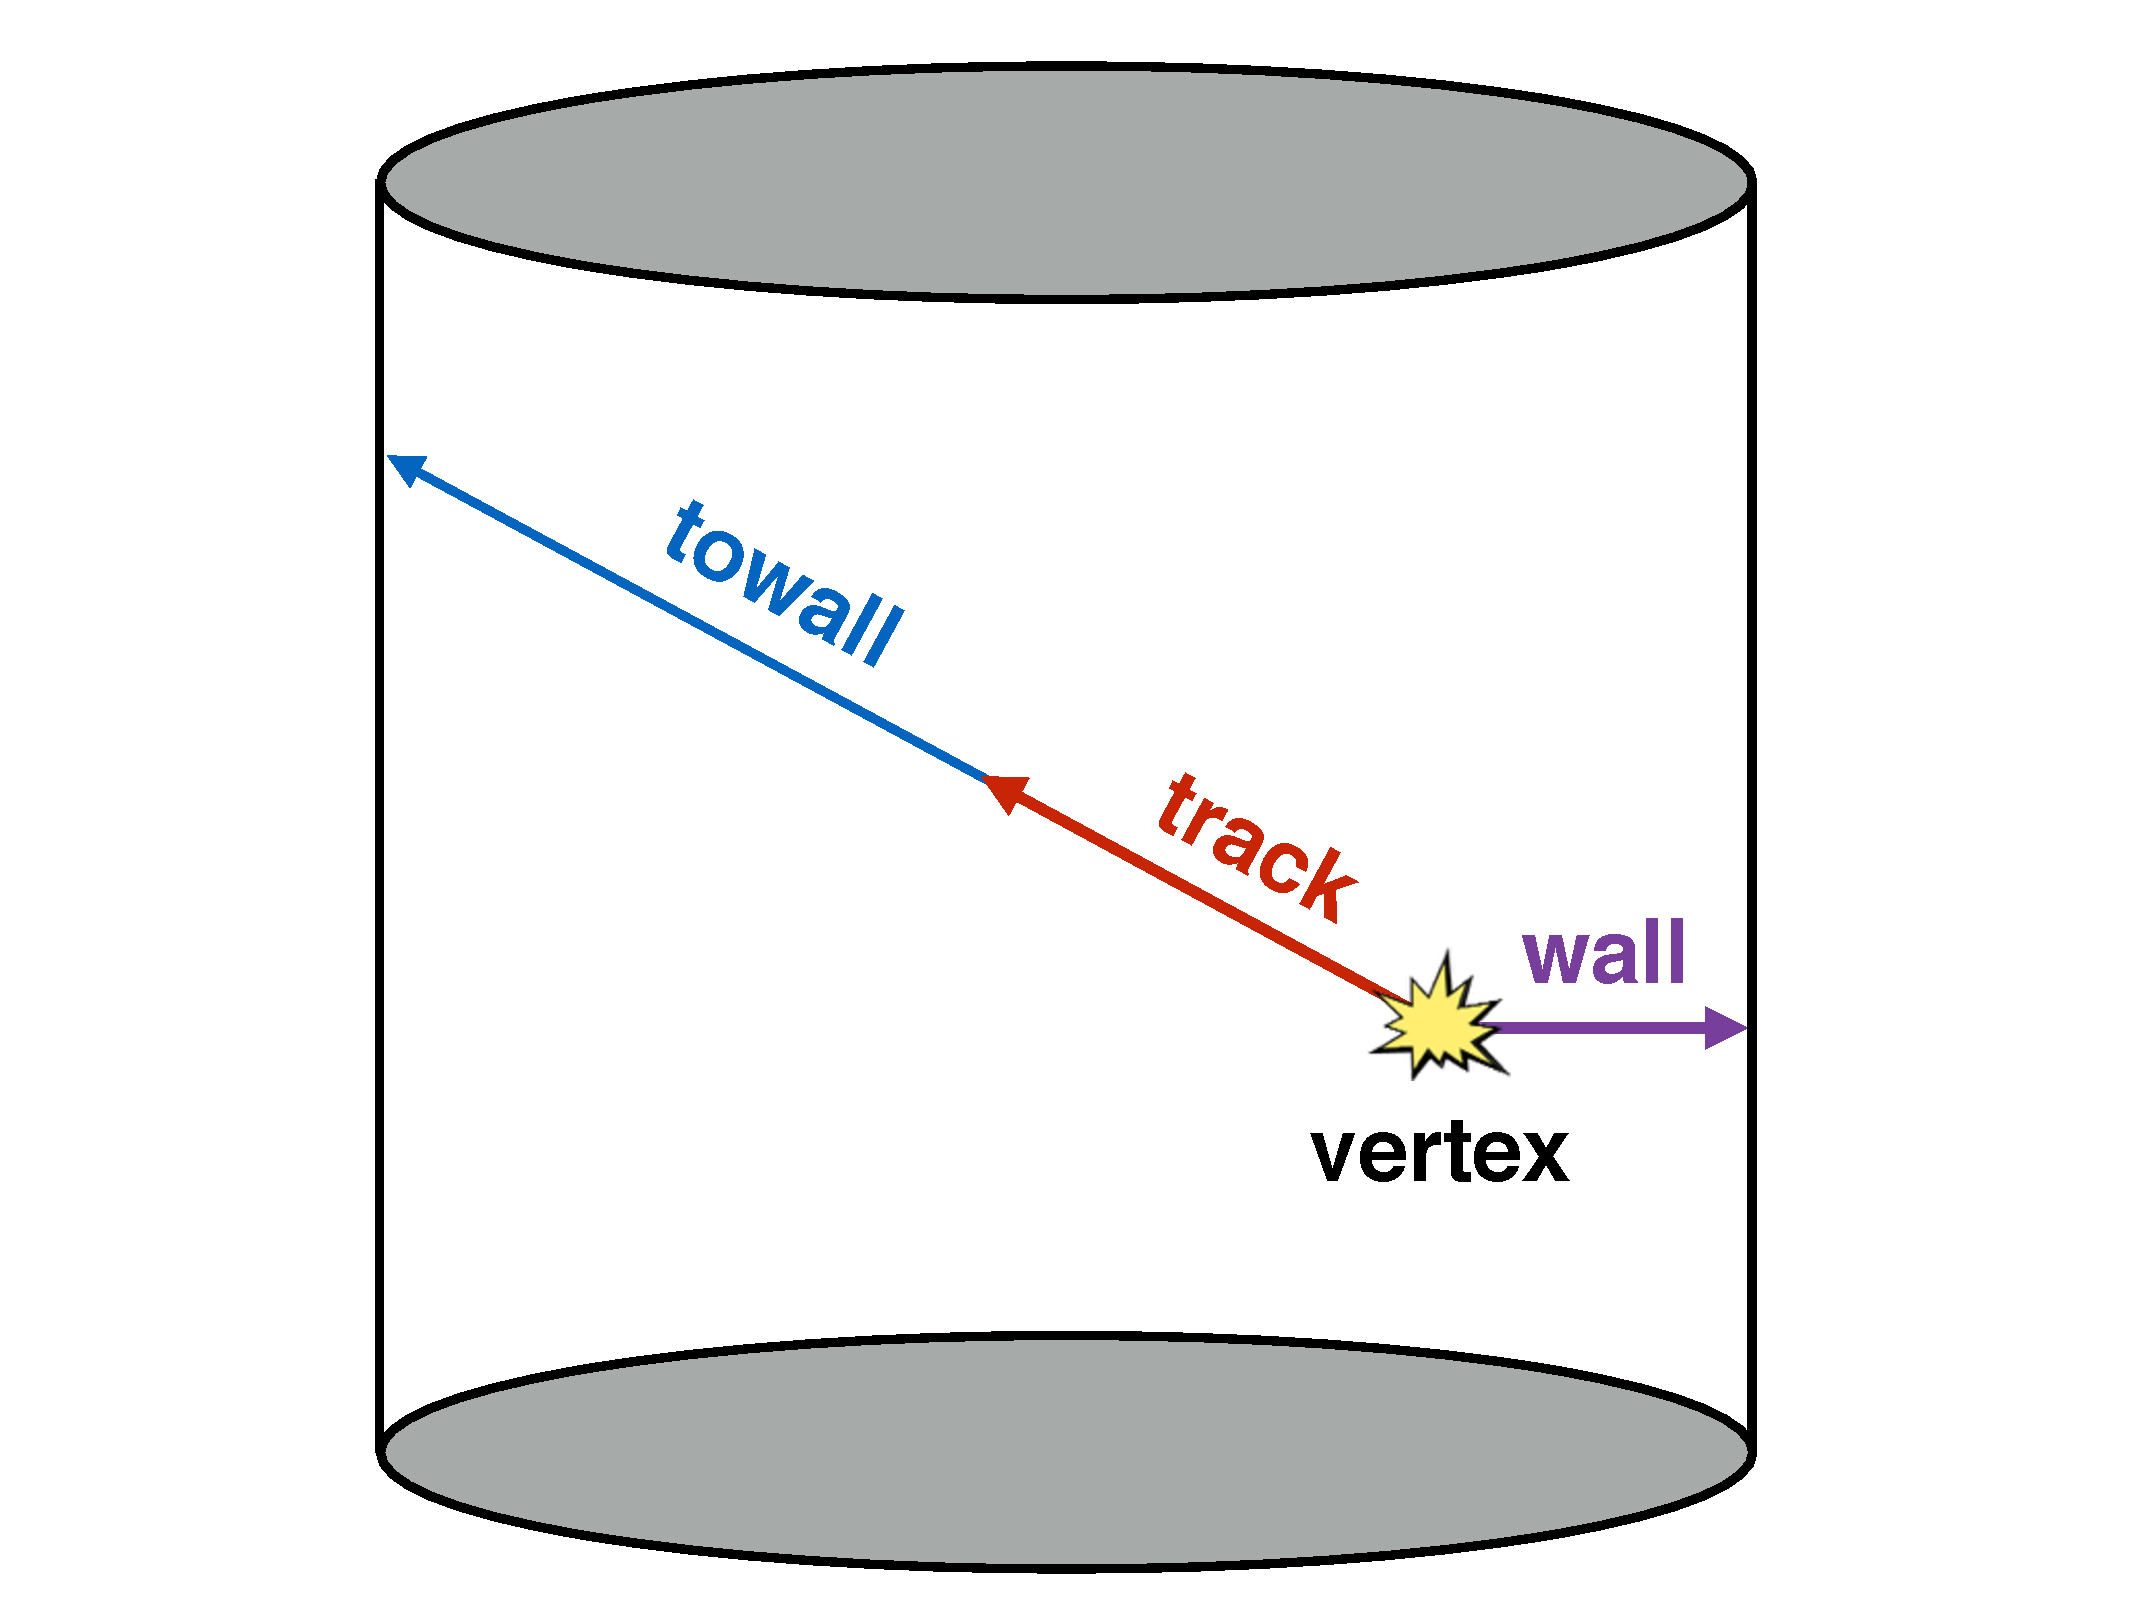
\includegraphics[width=0.5\textwidth]{wall_towall_def}
  \end{center}
  \caption{Graphical illustration of the definitions of the \wall and \towall variables
  that are cut on for the fiTQun FV cuts.  The \wall variable is the minimum distance between
  the reconstructed vertex and the ID wall, and the \towall variable is the distance along the 
  reconstructed particle track to the ID wall.}
  \label{fig:fvdiag}
\end{figure}

By discriminating events based on these two variables, we hope to better
isolate events that have poorly imaged Cherenkov rings from those with
well-imaged rings. Events that are close to the ID wall, but point inwards
(small \wall but large \towall), generally hit enough tubes to have a
well-imaged Cherenkov ring.  On the other hand, events that are close to the ID
wall but point towards the wall (small \wall and small \towall), generally hit
too few PMTS, and as a result have poorly imaged Cherenkov rings and may have to
be cut from the T2K sample.

\begin{table}
  \centering
  \begin{tabular}{c | c | c | c | c}
    \hline\hline
    Detector Region $j$ & Min. \towall & Max. \towall & Min. \wall & Max. \wall \\
    \hline\hline
    0 & 0cm    & 300  cm  & 0    cm & 300 cm \\
    1 & 300 cm & 5000 cm  & 0    cm & 80   cm \\
    2 & 300 cm & 800  cm  & 80   cm & 200 cm \\
    3 & 800 cm & 5000  cm & 80   cm & 200 cm \\
    4 & 300 cm & 800  cm  & 200  cm & 800 cm \\
    5 & 800 cm & 5000  cm & 200  cm & 5000 cm \\
    \hline\hline
  \end{tabular}
  \caption{Definitions of the detector region bins in terms of \wall and \towall.}
  \label{tab:fvbins}
\end{table}

\begin{figure}
  \begin{center}
    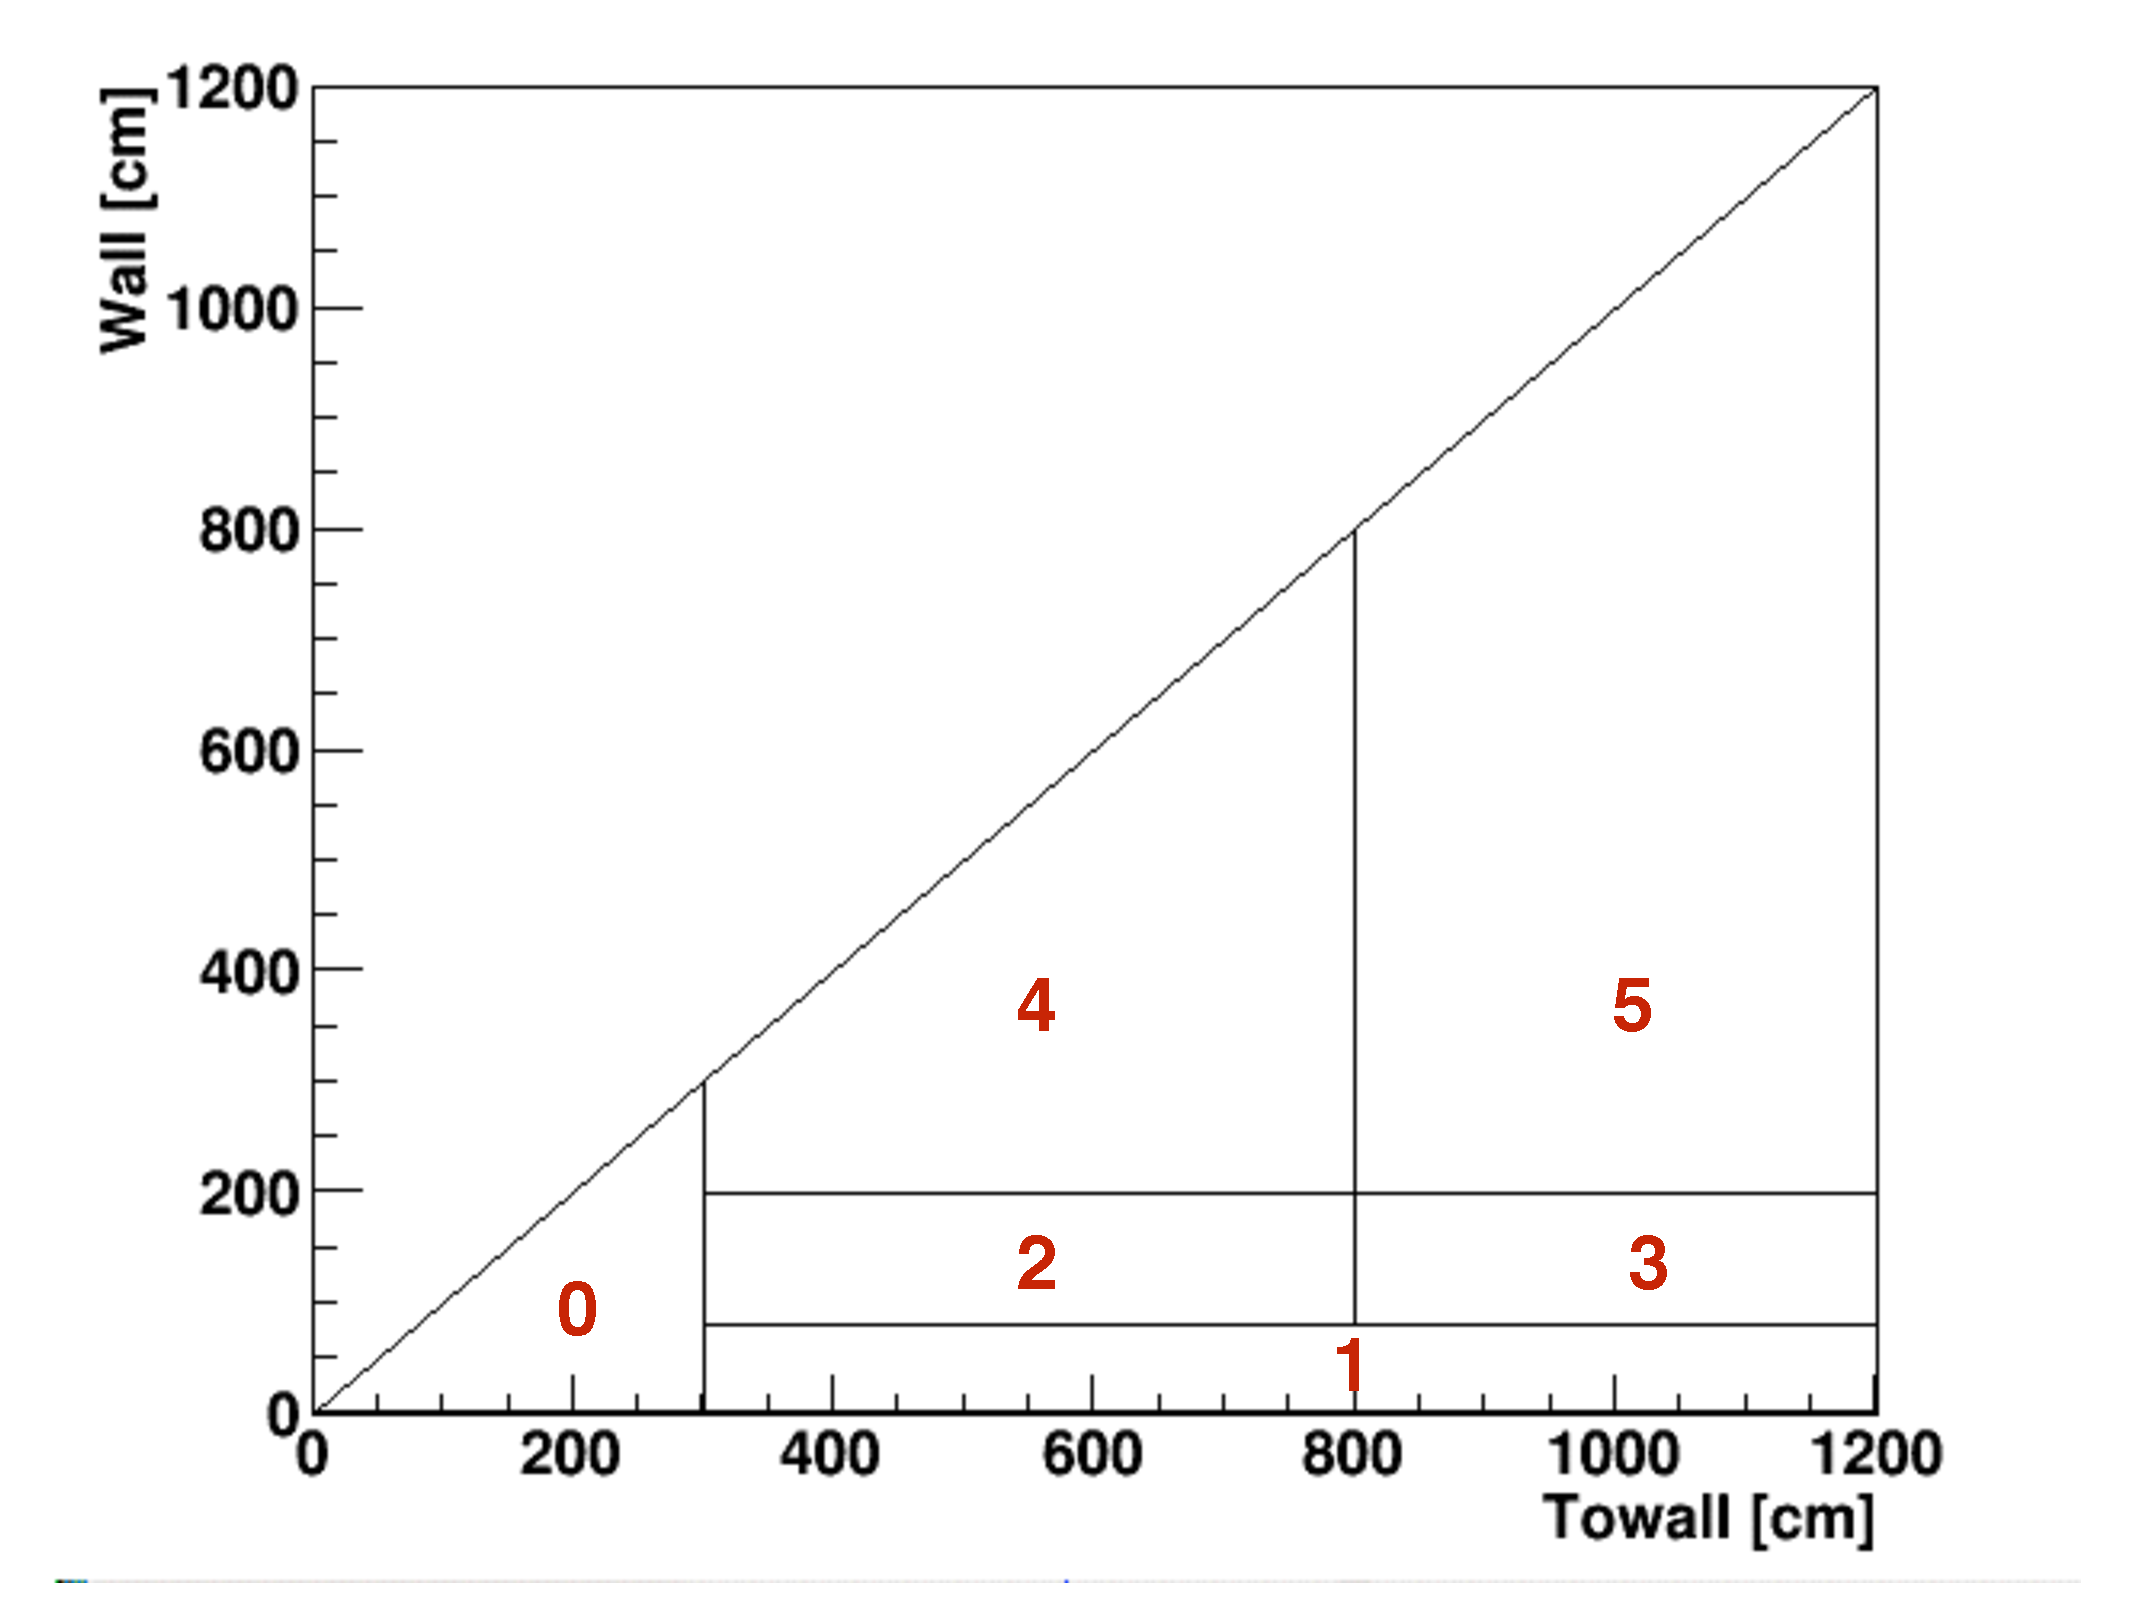
\includegraphics[width=0.5\textwidth]{plt_fvbins_labeled.pdf}
  \end{center}
  \caption{Graphical depiction of the detector region bins in terms of \wall
  and \towall.  Note that this plot is zoomed in on the small \wall and small
  \towall region.}
  \label{fig:fvbindef}
\end{figure}

A precise optimization of the fiTQun FV cuts requires knowledge of the SK
detector systematics in various regions of \wall and \towall.  To obtain this
information, we break up the $(towall,wall)$ space into bins and fit the
detector systematics in each bin separately.  The nominal binning in
\wall-\towall space is listed in Table~\ref{tab:fvbins} and shown in
Figure~\ref{fig:fvbindef}.  This binning was chosen to provide sensitivity to
how the systematic uncertainties change in key detector regions, while also
providing enough data statistics in each bin to constrain the parameters that
describe the uncertainties.  The events with both small \wall and small
\towall, (less than 300 cm) are isolated in the $j = 0$ FV bin.  Entering
background events, and events with poor energy reconstruction are almost
completely contained in the $j = 1$ FV bin.  The remaining region that with
\wall < 200cm is divided into two \towall bins.  Each bin in
Figure~\ref{fig:fvbindef} will receive an independent set of $\beta$ parameters
that describe the fiTQun distribution shapes as described in
Section~\ref{subsec:betapar}.




%-----------------------------------------------------------------------------
% Data Samples
%-----------------------------------------------------------------------------
\subsection{Data and MC Sample Definitions}
\label{subsec:samples}

The MC components described in Section~\ref{subsec:components} are obtained from
cuts on the true visible event topology.  To fit these different components to
the atmospheric data, we must define another set of cuts on reconstructed quantities
that can be applied to both data and MC simulation.  The goal is to 
separate out the differnt MC components, but ideally we should not
use the fiTQun cut variables (such particle ID or ring-counting) whose
uncertainties we are trying to measure.  We choose instead to break down the
data and MC into broad samples based on the number of decay electrons, as listed
in Table~\ref{tab:samples}.  The sample with no decay electrons emphasizes the
single ring electron component, while the single decay electron sample
emphasizes the single ring muon and multi-ring electron components. An
additional sample for multiple decay electrons emphasizes the multi-ring muon
components.  By dividing up the data and MC in this way, we hope to achieve better
resolution of the systematic error uncertainties for each individual component.
Examples of how the MC components are distributed in each sample can be seen in
Figure~\ref{fig:samplot0} through Figure~\ref{fig:samplot2}.

Since the shifts in the fiTQun likelihood distributions should be independent of the
number of sub-events, we do not assign independent systematic error parameters
based on these samples. Instead, we introduce an overall normalization
parameter for each sample, denoted as $\gamma_{j,l}$, that scales the total
number of events for the $l$-th sample in the $j$-th detector region bin.  The systematic 
uncertainties associated with the decay electron tagging efficiency have been
evaluated with a a separate study on stopping cosmic muon data and are
described in TN-217~\cite{tn317}.

\begin{table}
  \centering
  \begin{tabular}{c | c}
    \hline\hline
    Sample $l$ & Cut \\
    \hline
    1 & fqnse = 1 \\
    2 & fqnse = 2 \\
    3 & fqnse $>$ 2 \\
    \hline\hline
  \end{tabular}
  \caption{The sample cuts that are applied to both data and MC events. The
  fqnse variable is the number fiTQun sub-events. The number of decay electrons
  is $fqnse -1$. }
  \label{tab:samples}
\end{table}


\begin{figure}[h!]
\centering
\begin{tabular}{l  l  l}
  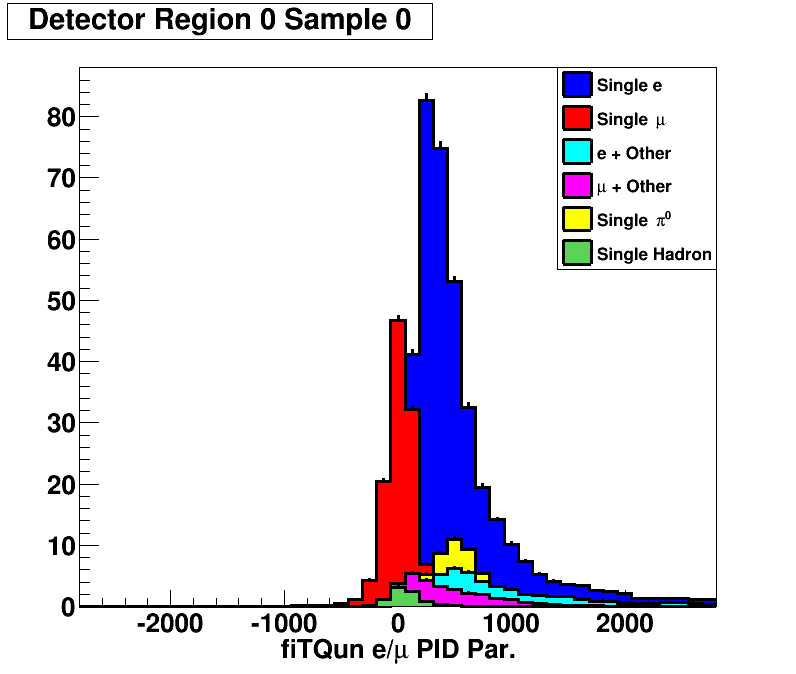
\includegraphics[width=0.33\textwidth]{plots/mc_breakdown_comp_0_bin_0_att_0} 
  &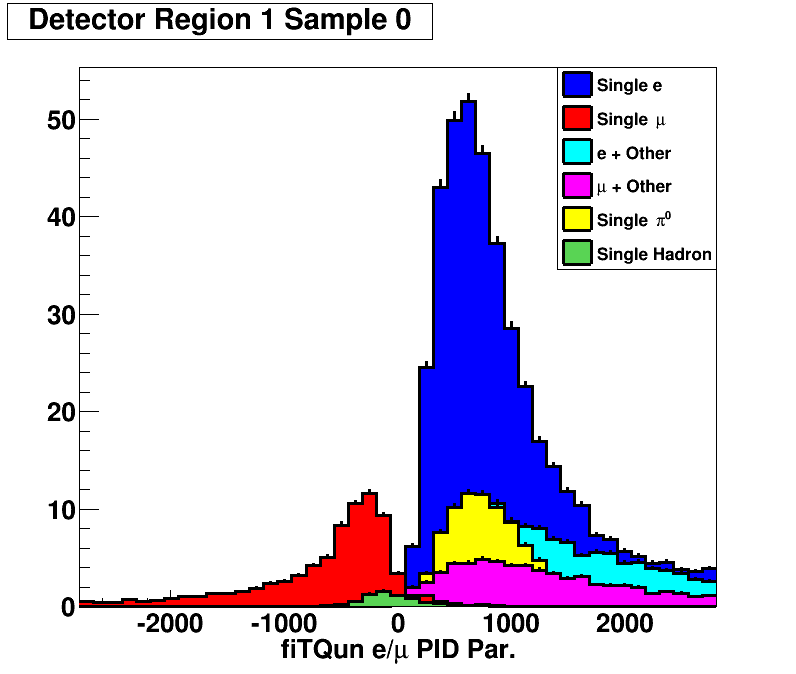
\includegraphics[width=0.33\textwidth]{plots/mc_breakdown_comp_0_bin_1_att_0}  
  &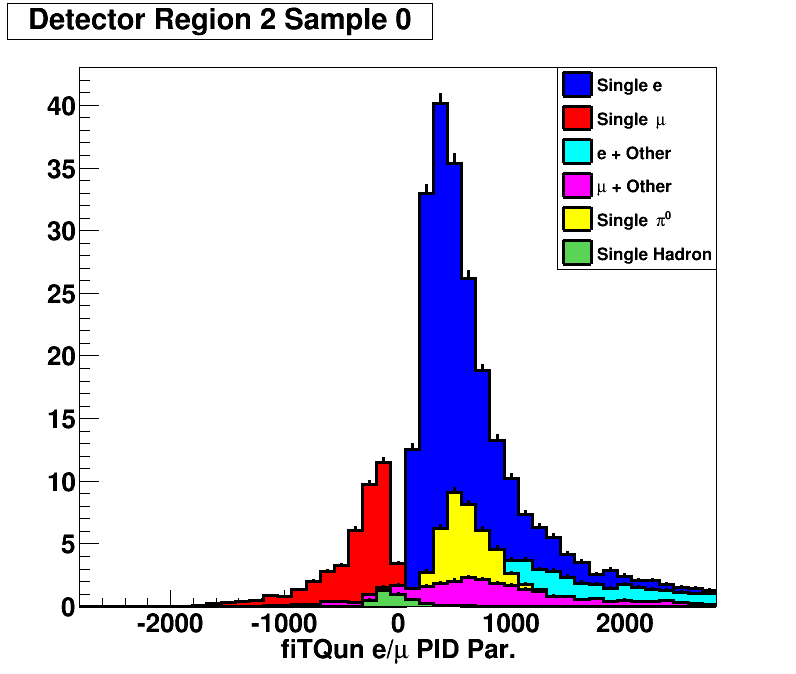
\includegraphics[width=0.33\textwidth]{plots/mc_breakdown_comp_0_bin_2_att_0} \\
  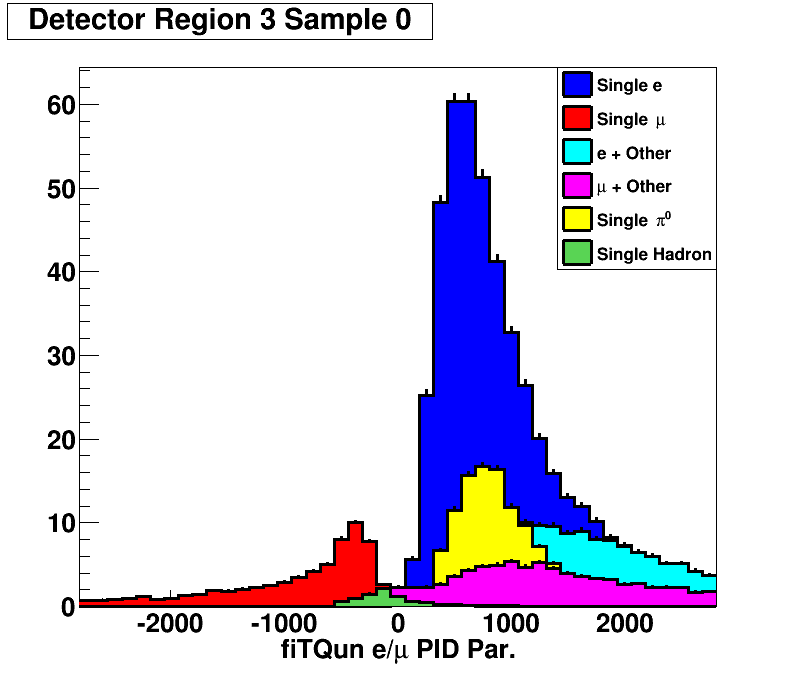
\includegraphics[width=0.33\textwidth]{plots/mc_breakdown_comp_0_bin_3_att_0} 
  &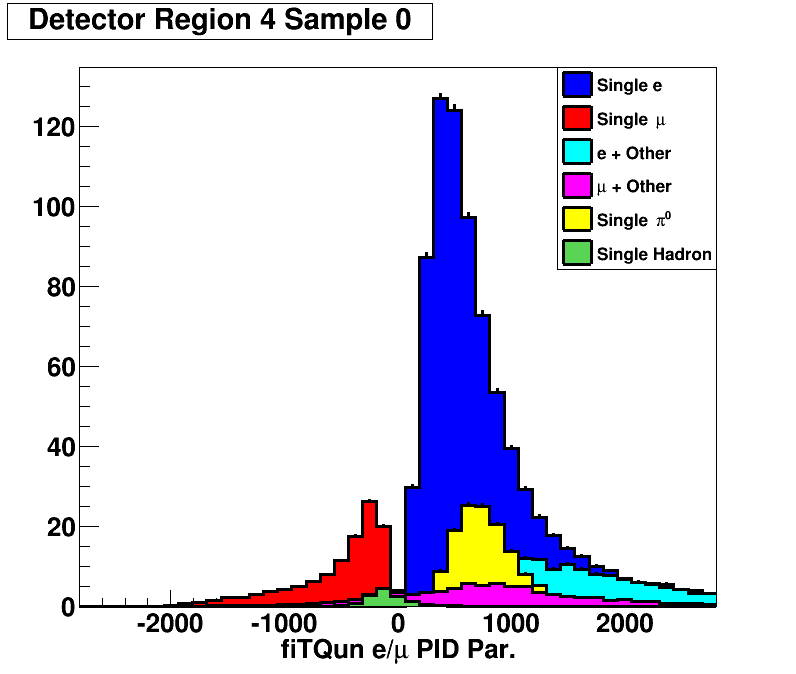
\includegraphics[width=0.33\textwidth]{plots/mc_breakdown_comp_0_bin_4_att_0} 
  &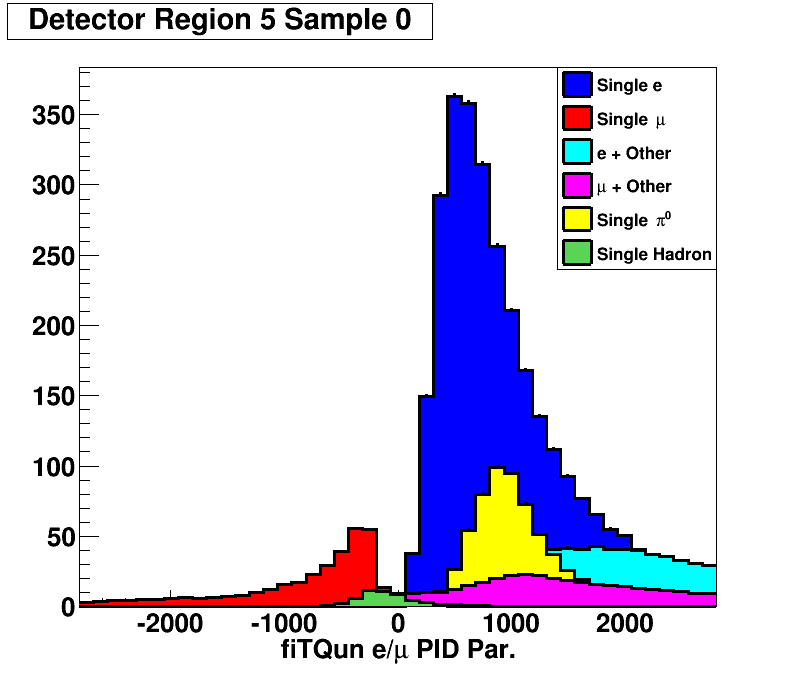
\includegraphics[width=0.33\textwidth]{plots/mc_breakdown_comp_0_bin_5_att_0}  
\end{tabular}
\caption{MC distributions of the fiTQun $e/\mu$ PID parameter for the $l = 0$
sample (no decay electrons) in all of the detector regions described in
Section~\ref{subsec:DR}.  In this sample, the single ring electron component
(defined in Section~\ref{subsec:components}) is emphasized. 
\towall.}
\label{fig:samplot0}
\end{figure}

\begin{figure}[h!]
\centering
\begin{tabular}{l  l  l}
  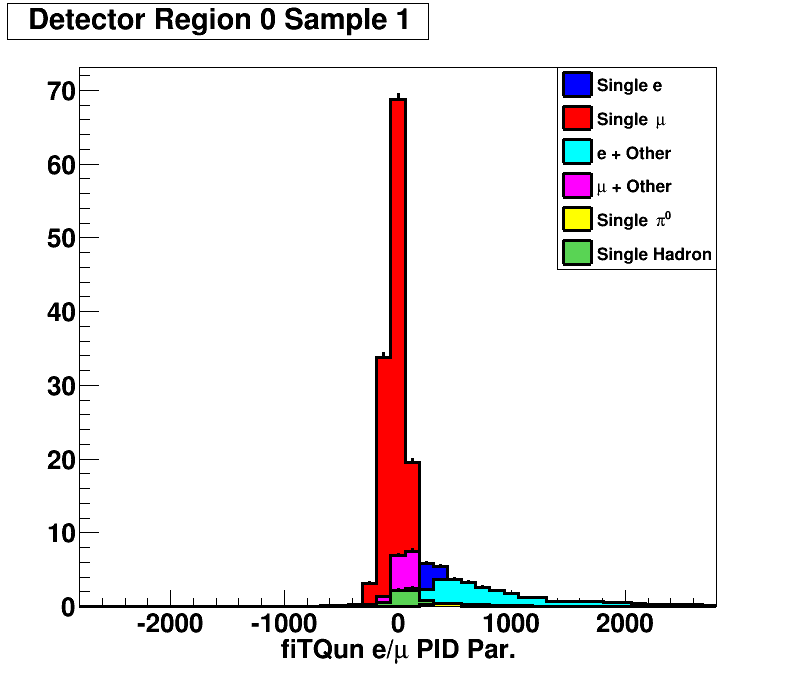
\includegraphics[width=0.33\textwidth]{plots/mc_breakdown_comp_1_bin_0_att_0} 
  &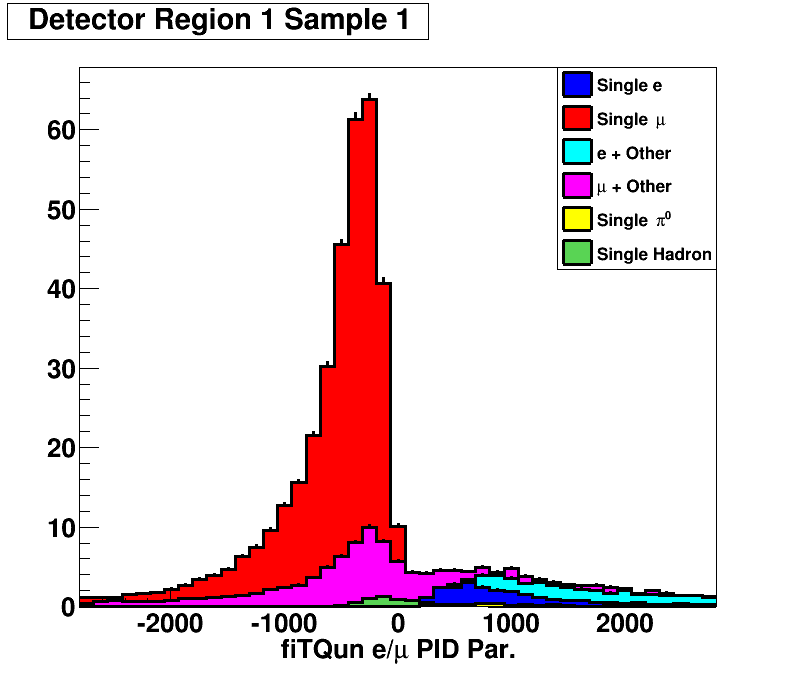
\includegraphics[width=0.33\textwidth]{plots/mc_breakdown_comp_1_bin_1_att_0}  
  &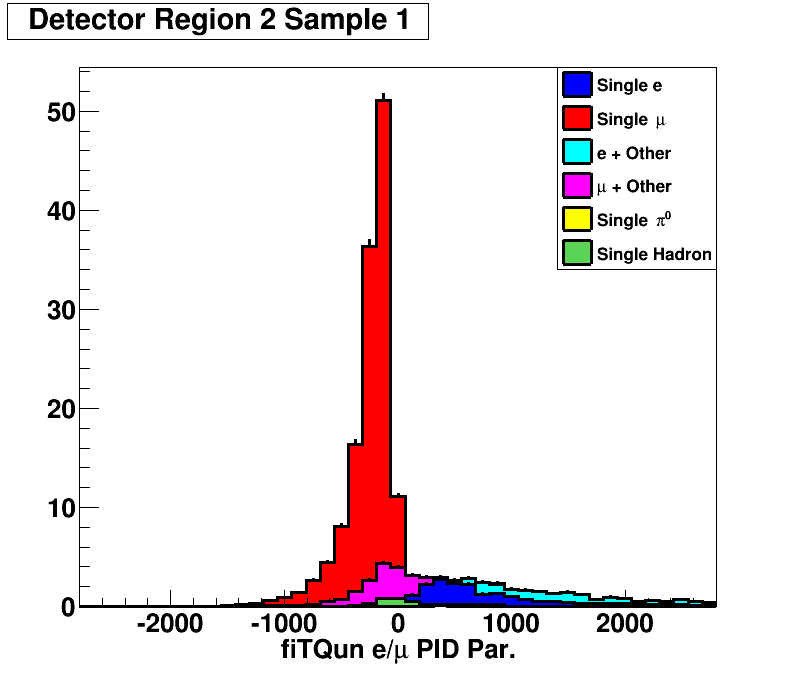
\includegraphics[width=0.33\textwidth]{plots/mc_breakdown_comp_1_bin_2_att_0} \\
  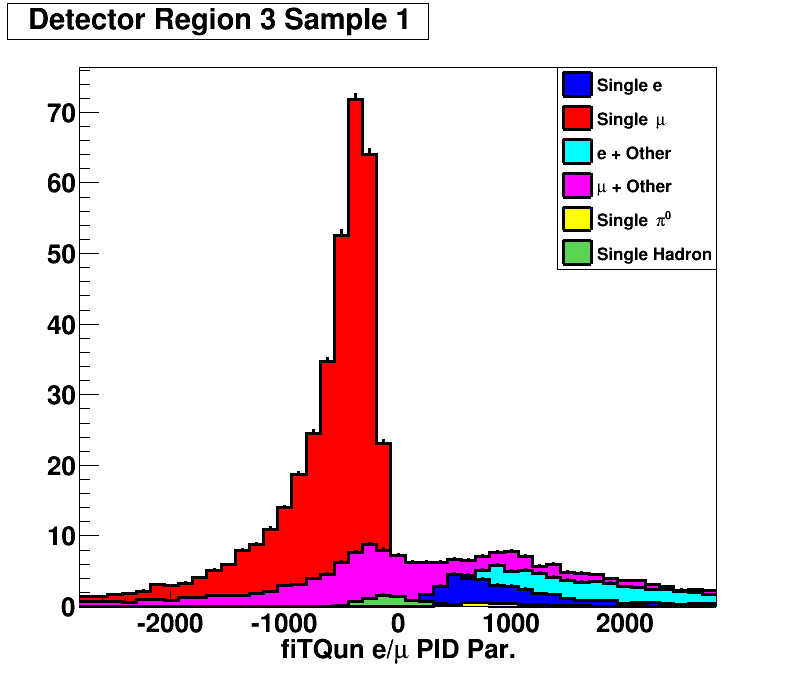
\includegraphics[width=0.33\textwidth]{plots/mc_breakdown_comp_1_bin_3_att_0} 
  &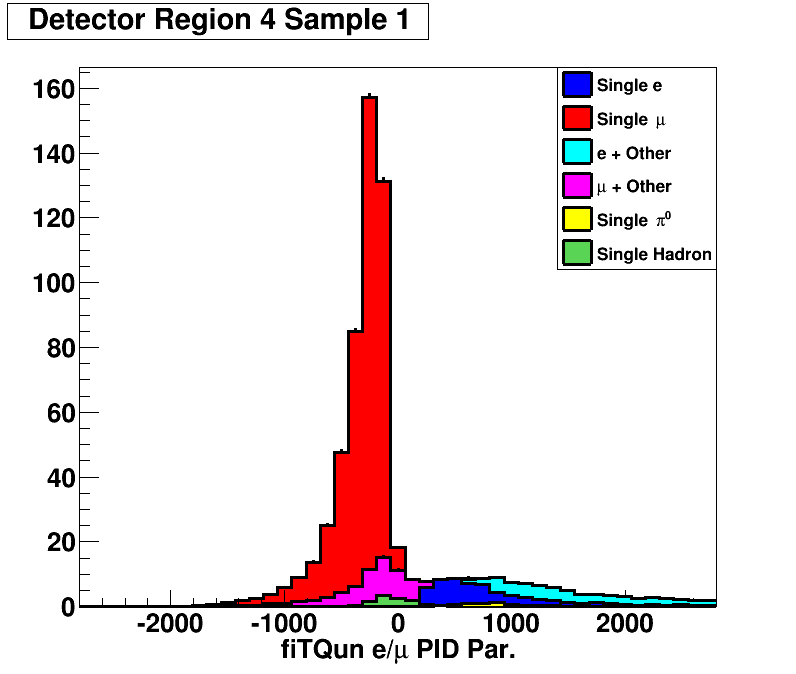
\includegraphics[width=0.33\textwidth]{plots/mc_breakdown_comp_1_bin_4_att_0} 
  &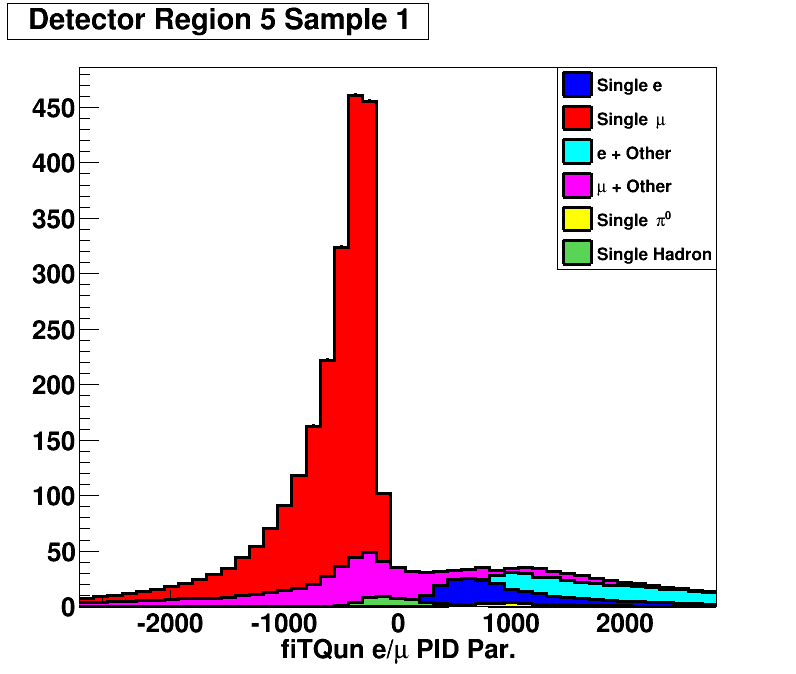
\includegraphics[width=0.33\textwidth]{plots/mc_breakdown_comp_1_bin_5_att_0} 
\end{tabular} 
\caption{MC distributions of the fiTQun $e/\mu$ PID parameter for the $l = 1$
sample (one decay electron) in all of the detector regions described in
Section~\ref{subsec:DR}.  In this sample, the single ring muon and multi-ring
electron components (defined in Section~\ref{subsec:components}) are
emphasized.}
\label{fig:samplot1}
\end{figure}

\begin{figure}[h!]
\centering
\begin{tabular}{l  l  l}
  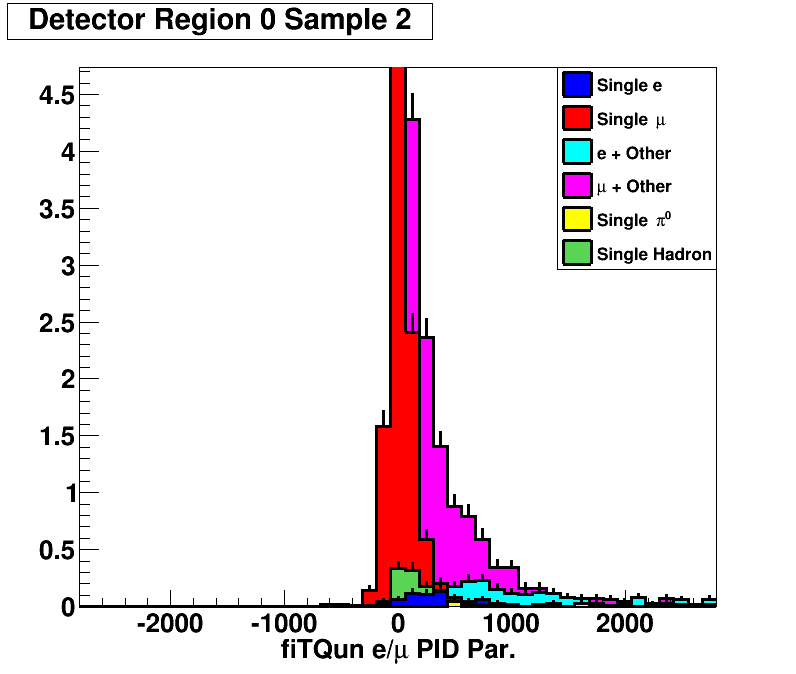
\includegraphics[width=0.33\textwidth]{plots/mc_breakdown_comp_2_bin_0_att_0} 
  &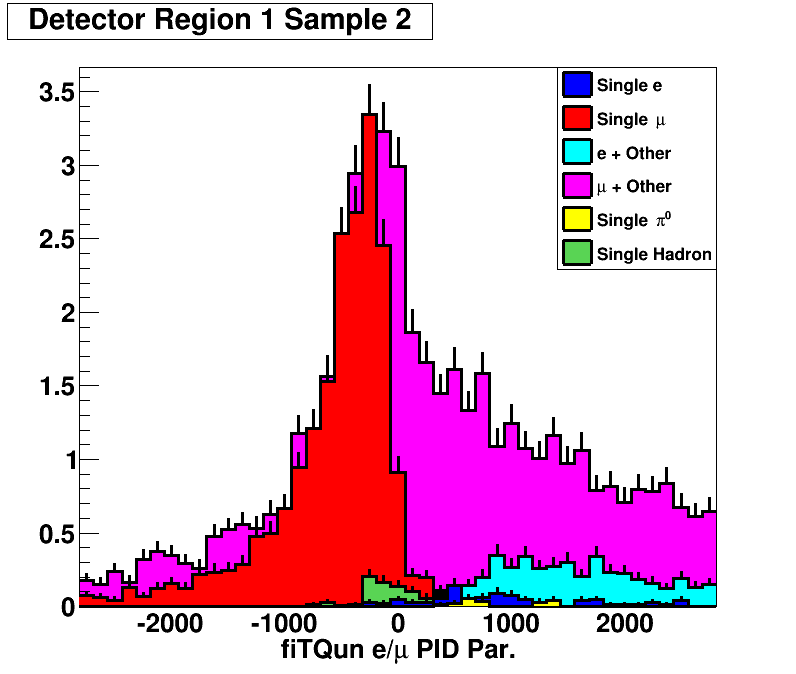
\includegraphics[width=0.33\textwidth]{plots/mc_breakdown_comp_2_bin_1_att_0}  
  &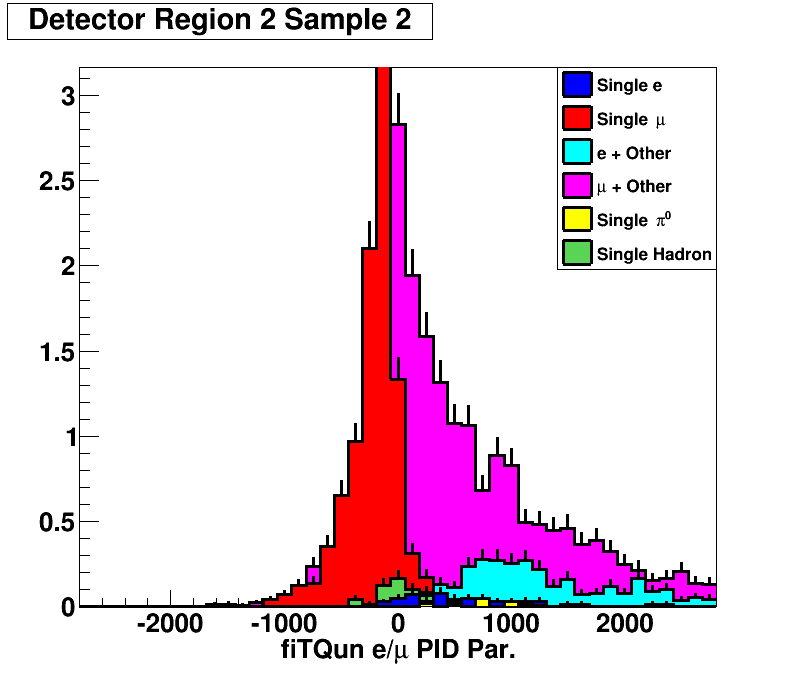
\includegraphics[width=0.33\textwidth]{plots/mc_breakdown_comp_2_bin_2_att_0} \\
  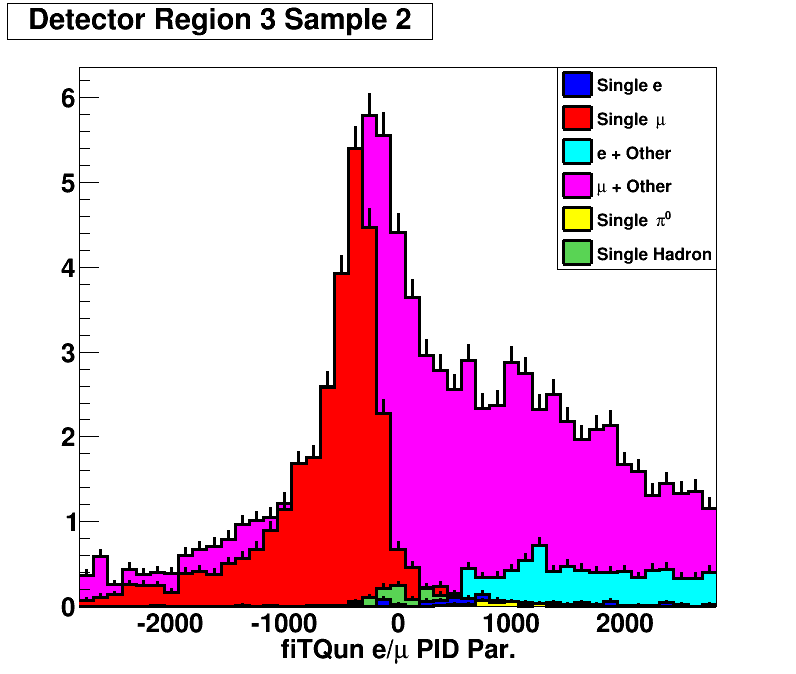
\includegraphics[width=0.33\textwidth]{plots/mc_breakdown_comp_2_bin_3_att_0} 
  &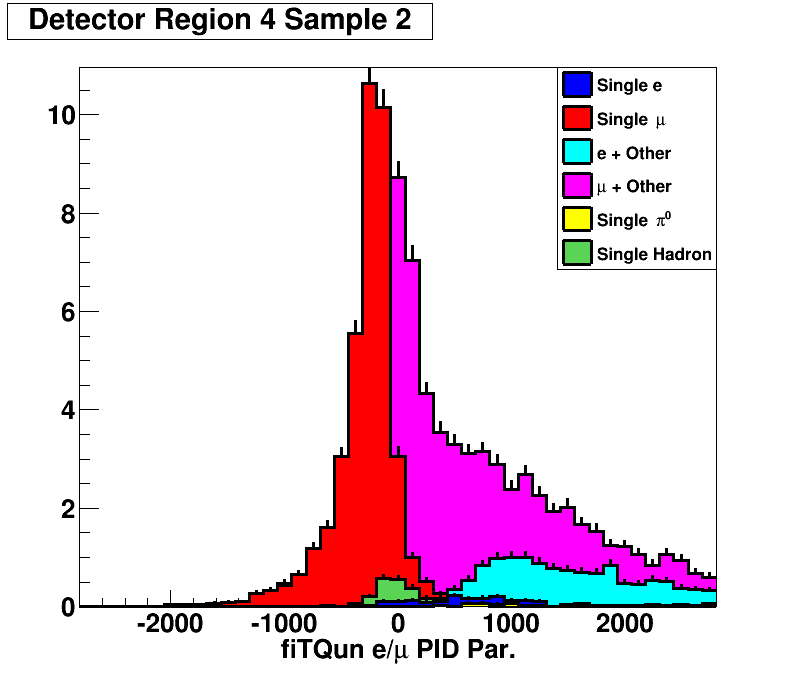
\includegraphics[width=0.33\textwidth]{plots/mc_breakdown_comp_2_bin_4_att_0} 
  &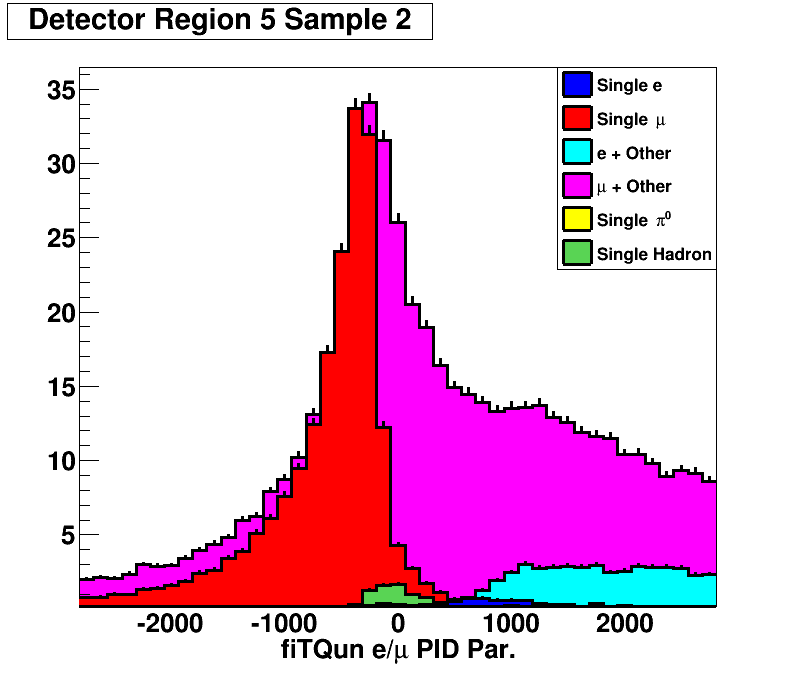
\includegraphics[width=0.33\textwidth]{plots/mc_breakdown_comp_2_bin_5_att_0} 
\end{tabular} 
\caption{MC distributions of the fiTQun $e/\mu$ PID parameter for the $l=2$ 
sample (more than one decay electron) in all of the detector regions described in
Section~\ref{subsec:DR}.  In this sample, the multi-ring muon component
(defined in Section~\ref{subsec:components}) is emphasized.}
\label{fig:samplot2}
\end{figure}
\FloatBarrier




%-----------------------------------------------------------------------------
% Full Parameterization
%-----------------------------------------------------------------------------
\subsection{Full Fit Parameterization}
\label{subsec:fullpars}

The full parameterization for the atmospheric fit is defined in terms of the MC
components, the detector regions, and the flux and cross section parameters
described in the previous sections.  The fiTQun cut variables we wish to
estimate systematics for are listed in Table~\ref{tab:fqvars}. The full
parameterization of the detector systematics is then the following set of
parameters:

\begin{equation}
  \label{eq:fullpars}
  \{\alpha_{n}, \beta_{j,k,m}^{i}, \gamma_{j,l} \}
\end{equation}

Where $i \in \{0,1\}$ denotes the additive or multiplicative shape parameter
described in Section~\ref{subsec:betapar}, $j \in \{0,1,2,3,4,5\}$ denotes the
detector region bin, $k \in \{0,1,2,3,4,5\}$ denotes the MC component described
in Section~\ref{subsec:components},  $l \in \{0,1,2\}$ denotes the sample
described in Section~\ref{subsec:samples}, and $m \in \{0,1,2,3\}$ denotes the
fiTQun cut variable in Table~\ref{tab:fqvars}. 

There are 288 of the $\beta$ parameters in total.  These parameters are fit
simultaneously with the atmospheric flux and cross section parameters
$\alpha_{n}$ (19 parameters) and the sample normalizations $\gamma_{j,l}$ (18
parameters) for a total of 325 parameters in this fit.



%-----------------------------------------------------------------------------
% Likelihood Definition
%-----------------------------------------------------------------------------
\subsection{Parameter Likelihood Definition}
\label{subsec:parlike}

With the fit parameters described in previous sections, we now address the
details of how they are constrained by the SK atmospheric neutrino data.  In
previous atmospheric fits, such as the one described in TN-186, the parameters
are constrained by comparing the numbers of events that either pass or fail the
cuts on the reconstructed variables.  This amounts to essentially binning each
of the cut variables into two bins separated by the optimal cut chosen for the
T2K analysis.  We modify this approach by fitting to the full distributions
of the fiTQun cut variables listed in Table~\ref{tab:fqvars}.

There are several advantages to fitting to the entire cut variable
distributions.  One clear advantage is that this includes more shape
information in the fit, which should in principle provide better constraints on
the systematics for the MC components that dominate each distribution. This
point is particularly important for determining systematics in the small \wall
and small \towall detector regions, where the data statistics becomes a limiting
factor.  Another advantage is that this decouples the estimation of detector
systematics from the optimization of the cut values, since we no longer use the
T2K cut values explicitly in the fit.   

To formalize this concept, we define $\mathbf{h}^{MC}$ to be the set of
histograms $h^{MC}_{j,l,m}$ filled from MC for all values of $j$, $l$, and $m$,
where again $j$  is the detector region bin, $l$ is the sample based on the
number of decay electrons, and $m$ is the index of the fiTQun topological cut
variable from Table~\ref{tab:fqvars}.

Similarly, we define $\mathbf{h}^{Data}$ as the set of histograms
$h^{Data}_{j,l,m}$ filled using SK atmospheric data. We consider $
\mathbf{h}^{Data}$ to be the observed data $\mathbf{M}_{Atm-Sk}$ in
Equation~\ref{eq:likelihood}, and the previously defined detector systematic
parameter sets $\beta$, and normalizations $\gamma$ to be \ldsk, and finally
the flux and cross section parameters $\alpha$ from
Section~\ref{subsec:alphapar} to be $\mathbf{a}$ and $\mathbf{x}_{atm}$.  We can now define the
negative log-likelihood from Equation~\ref{eq:likelihood} to be:
%
\begin{equation}
  \label{eq:loglikelihood}
  -log[\mathcal{L}(\alpha,\beta,\gamma | \mathbf{h}^{Data} )] =
  -log[P( \mathbf{h}^{Data} | \mathbf{h}^{MC}(\alpha,\beta,\gamma))] - log[\pi(\alpha)]
  - log[\pi(\beta,\gamma)]
\end{equation}
%
The first term on the right hand side can be expanded as a sum over the bins
$s$, assuming Poisson statistics in each bin:
%
\begin{gather*}
  \label{eq:logpoisson}
  -log[P( \mathbf{h}^{Data} | \mathbf{h}^{MC}(\alpha,\beta,\gamma))] = \\
    \sum\limits_{s}^{} \sum\limits_{j}^{} \sum\limits_{l}^{} \sum\limits_{m}^{} 
   \bigg[ (\hat{N}_{s,j,l,m}(\alpha,\beta,\gamma) - N_{s,j,l,m}) +
  N_{s,j,l,m}log\bigg(\frac{N_{s,j,l,m}}{\hat{N}_{s,j,l,m}(\alpha,\beta,\gamma)}\bigg)\bigg]
\end{gather*}
%
where $N_{s}$ denotes the observed contents of the histogram bin $s$, and
$\hat{N}_{s}$ denotes the MC expectation (assumed to be the Poisson mean) of
histogram bin $s$ given the values of the systematics parameters.  The
histogram bin widths, as well as the maximum and minimum values of the
histogram $x$-axis, were chosen to obtain reasonable data statistics in each
bin, as well as to emphasize the regions near the T2K cut values, where any
shift will have the largest impact on the size and composition of the event
samples.  The exact histogram ranges and bin size can be seen most readily in 
Figures~\ref{fig:fitresults_samp0_att0}-~\ref{fig:fitresults_samp2_att3} found in 
Section~\ref{sec:fitresults}.

The remaining terms in the likelihood are the priors for each of the fit
parameters.  We assume each prior is a Gaussian shape with some width
$\sigma$ around the nominal parameter values.  For the atmospheric flux and
cross section parameters $\alpha$, we take $\sigma_{\alpha_{n}}$ to be the
values listed in Table~\ref{tab:alpha}.  For the detector systematics
parameters $\beta$ we assign the priors listed in Table~\ref{tab:betaprior}.
These priors are chosen to provide a loose constraint that does not dominate
over the constraints from data, but also to keep the parameters constrained
from moving to values that are much more extreme values.  We can then expand
the terms for the priors as:
%
\begin{gather*}
  \label{eq:logpriors}
  - log[\pi(\alpha)] - log[\pi(\beta,\gamma)] = \\ \frac{1}{2}
  \sum\limits_{n}^{} \bigg(\frac{(\alpha_{n} - 1)}{\sigma_{\alpha_{n}}}\bigg)^{2} +
   \frac{1}{2} \sum\limits_{j}^{} \sum\limits_{l}^{} 
  \bigg(\frac{(\gamma_{j,l} - 1)}{\sigma_{\gamma_{j,l}}}\bigg)^{2} + 
   \frac{1}{2} \sum\limits_{i}^{} \sum\limits_{j}^{} \sum\limits_{l}^{} \sum\limits_{m}^{}
  \bigg(\frac{(\beta_{j,l,m}^{i} - \delta_{i1})}{\sigma_{\beta_{m}}}\bigg)^{2}  
\end{gather*}
%
Putting of this all together, we wish to minimize the following negative log-likelihood, which is a
sum of $1,134$ terms:
%
\begin{equation}
 \begin{gathered}
  -log[\mathcal{L}(\alpha,\beta,\gamma | \mathbf{h}^{Data}  )] = \\
  \sum\limits_{s}^{} \sum\limits_{i}^{}  \sum\limits_{j}^{} \sum\limits_{l}^{} \sum\limits_{m}^{} \sum\limits_{n}^{}
  \bigg[ (\hat{N}_{s,j,l,m}(\alpha,\beta,\gamma) - N_{s,j,l,m})
    + N_{s,j,l,m}log\bigg(\frac{N_{s,j,l,m}}{\hat{N}_{s,j,l,m}(\alpha,\beta,\gamma)}\bigg) \\
  + \frac{1}{2}\bigg(\frac{(\alpha_{n} - 1)}{\sigma_{\alpha_{n}}}\bigg)^{2}
  + \frac{1}{2}\bigg(\frac{(\gamma_{j,l} - 1)}{\sigma_{\gamma_{j,l}}}\bigg)^{2} 
  + \frac{1}{2}\bigg(\frac{(\beta_{j,l,m}^{i} - \delta_{i1})}{\sigma_{\beta_{m}}}\bigg)^{2} \bigg] 
 \end{gathered}
 \label{eq:likefull}
\end{equation}


\begin{table}[h]
  \centering
  \begin{tabular}{c|c|c}
   \hline\hline
   $m$ & fiTQun Variable Name & Prior Constraint $\sigma_{\beta_{m}}$ \\
   \hline\hline
   0 & $e/\mu$ PID & 200 \\
   1 & $e/\pi^{0}$ PID & 200 \\
   2 & $\mu/\pi$ PID & 200 \\
   3 & Ring-Counting &100 \\
   \hline\hline
  \end{tabular}
  \caption{Loose prior constraints assigned to the detector systematics parameters. The
  constraint values are dimensionless and reflect the scales of the fiTQun likelihood ratios
  for each variable.}
  \label{tab:betaprior}
\end{table}




%-----------------------------------------------------------------------------
% Likelihood Evaluation 
%-----------------------------------------------------------------------------
\subsection{Likelihood Evaluation}
\label{subsec:evalike}

While perhaps formally imposing, the likelihood defined explicitly in
Equation~\ref{eq:likefull} simply compares the data and MC by chopping the
events up into many histograms and then comparing data and MC in each bin.
This can be calculated numerically in a straightforward manner:

\begin{enumerate}
  \item \label{it:first} Fill a set of histograms of the fiTQun cut variables using the atmospheric data.
    There is a histogram for each cut variable, each detector region,
    and each control sample defined by the number of decay electrons.
  \item
    Fill a separate set of histograms using simulated data for some assumed
    values of the $\alpha$, $\beta$, and $\gamma$ parameters. There is a
    histogram for each fiTQun cut variable, each detector region, each control
    sample, \emph{and} each component defined by the true visible topology
  \item \label{it:sum} Sum the histograms of the MC components for each cut
    variable, each detector region, and each control sample. The resulting summed histograms
    does not depend on MC truth information and can be compared directly to data.
  \item
    \label{it:comp} Compare the MC summed histogram from Step~\ref{it:sum} to
    the corresponding data histogram, by evaluating the log-likelihood bin-wise
    as in Equation~\ref{eq:logpoisson}. 
  \item Add the contributions from the
    priors to the result of Step~\ref{it:comp} to obtain the final likelihood
    value from Equation~\ref{eq:likefull}.
\end{enumerate}

The steps outlined above can be repeated for different assumptions of the
systematics parameters to compare the relative likelihood of different
assumptions of systematics.  The goal now is to find the parameters that give
the best agreement to the data, i.e.\ the parameters that minimize the negative
log-likelihood.  Ideally, we would like to know not only the best-fit parameter
values, but also the preferred parameter regions and correlations.  To
accomplish this task, we use Markov chain Monte Carlo (MCMC) methods.



%-----------------------------------------------------------------------------
% MCMC Fit Methods
%-----------------------------------------------------------------------------
\subsection{MCMC Methods}
\label{subsec:mcmc}

MCMC is a stochastic technique that can be used to generate samples of detector
systematic parameters drawn from the likelihood defined in
Equation~\ref{eq:likefull}.  This is accomplished by essentially taking a
random walk through the parameter space and preferentially accepting steps
according to the likelihood definition. If we let $\theta$ denote the full set
of fit parameters, i.e.\ $\theta = (\alpha,\beta,\gamma)$, a MCMC run of length
N will produce a set of parameter values: $\{\theta_{1}, \theta_{1}, \dots
\theta_{N}\}$.  We can the sample from this set to obtain approximately
independent throws from the likelihood, which provides a powerful tool for
propagating uncertainties.  This is due to the fact that if we have some
quantity $X$ that depends on $\theta$ (such as the number of events passing
some set of selection criteria), we can easily calculate the expectation over
$\theta$ as as an average over some number $M$ of MCMC points:
%
\begin{equation}
  \label{eq:mcmcexp}
  \langle X \rangle_{\theta} = \frac{1}{M}\sum\limits_{i=0}^{M}X(\theta_{i})
\end{equation}
%
This expectation can then be compared to the nominal simulated value of $X$ to
quote a systematic uncertainty.

The MCMC in this fit uses the Metropolis-Hastings algorithm, described
in detail in the PDG and TN-140.  The procedure is as follows:

\begin{enumerate}
  \item Determine a distribution $Q(\theta|\theta_{0})$ that assigns a
    probability to each point $\theta$ given the current point $\theta_{0}$.
    This distribution should be symmetric under exchange of $\theta$ and
    $\theta_{0}$ so that $Q(\theta|\theta_{0}) = Q(\theta_{0}|\theta) $
  \item Choose an initial point  $\theta_{0}$
  \item Randomly select a proposed step according to $Q(\theta|\theta_{0})$.
  \item Calculate an acceptance probability $\Omega = min(1,\frac{P(\theta)}{P(\theta_{0})})$.
  \item Randomly select a point $u \in \{0, 1\}$ according to a uniform distribution.
  \item If $u<\Omega$, accept this proposal and return to Step 1 with $\theta_{0} = \theta$ 
  \item If $u>\Omega$, reject this proposal and return to Step 1 with $\theta_{0} = \theta_{0}$ 
\end{enumerate}

In practice, we first select an initial starting point $\theta_{0}$ by
minimizing the likelihood using MINUIT\@.  We then profile the likelihood for
each fit parameter $\theta^{i}$ to obtain a rough estimate of how sensitive the
likelihood is to changes in $\theta^{i}$.  The width of this likelihood profile
is then used to build a proposal distribution $Q(\theta|\theta_{0})$ that
throws each parameter independently from a Gaussian distribution centered on
$\theta^{i}_{0}$ and with a width determined by the 1D likelihood profile.

One potential drawback of using the proposal distribution
$Q(\theta|\theta_{0})$ described above is that it treats all parameters
independently and ignores potential correlations between the parameters.  In
the limit of infinite MCMC steps, this is not a problem, since the proposal
function will eventually ``guess'' all of the parameter combinations.  With a
finite chain, however, the presence of strong correlations between the fit
parameters may result in the chain not fully exploring the space of allowed
parameters, since some specific combinations that agree well with the data may
end up not be sampled by the proposal function in time.

The issue of strongly correlated parameters is particularly problematic for
this analysis due to our choice of detector error parameterization.  By
examining how the $\beta$ parameters are applied (see
Equation~\ref{eq:fqparmod}), it is clear that if the fiTQun variable $L_{m}$ is
not distributed around $0$, then a change in the multiplicative parameter
$\beta^{1}$ will also produce a shift which modifies the distribution in the
same manner as a change in $\beta^{0}$.  This redundancy results in strong
correlations between the $\beta^{0}$ and $\beta^{1}$ parameters.

One way to deal with this issue is to modify the proposal function to include
the expected parameter correlations.  There are many ways to approach this
problem, but one elegant way is to borrow the ideas from Differential Evolution
Markov Chain Monte Carlo (DE-MCMC).  A description of the algorithm can be
found in, for example, the Braak2006~\cite{Braak2006}. The strategy adopted
here is to run an initial MCMC and record the difference $\Delta \theta$ in the
parameters between each accepted point and some previously accepted point. The
result is a sampling of the preferred directions in the parameter space. One
can then sample from this list of preferred directions to build a proposal
function that includes all of the relevant correlations.  The overall approach
is as follows:
%
\begin{enumerate}
  \item Run an initial Metropolis-Hastings MCMC to obtain a set of the
    accepted point differences.  
  \item Choose a random element $\Delta \theta$ from the set of accepted point
    differences generated in Step 1.
  \item Choose a random perturbation $\delta$ (should be small compared to the characeristic
    $\Delta \theta$ step size).
  \item Given some initial point $\theta_{0}$ propose the next point $\theta$
    according to: $\theta = \theta_{0} + a \Delta \theta + \delta$. Where $a$ is some scaling factor that is
    tuned so the accpetance rate is $\approx 0.25$.
\end{enumerate}
%
By defining the proposal function in this way, we are able to sample from the
parameter space much more efficiently. This results in the MCMC converging much
more quickly to the paramters that minimize the likelihood, as can been seen in
Figure~\ref{fig:burnin}.


\begin{figure}[h]
  \begin{center}
    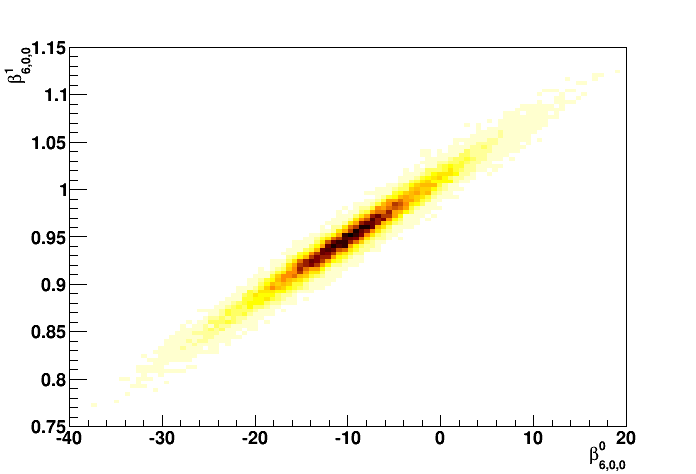
\includegraphics[width=0.5\textwidth]{corr_example}
    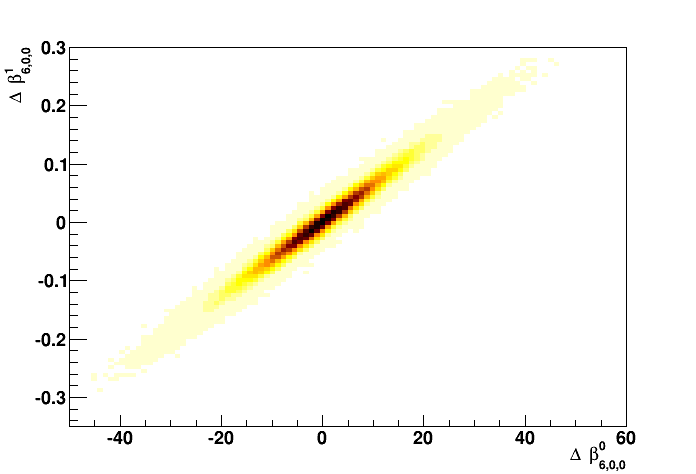
\includegraphics[width=0.5\textwidth]{diff_example}
  \end{center}
  \caption{Upper plot shows the histogram of the MCMC points for the
  multiplicative and additive parameters that affect the shape of the
  single-ring electron $e/\mu$ PID variable in Detector Region 6.  Note
  the strong correlations between the two parameters coming from the fact that
  the effects of varying these parameters partially cancel.  Lower plot shows
  the histogram of the accpeted parameter differences.  The DE-MCMC method
  draws from the lower distribution to better sample these correlated parameters.}
  \label{fig:parcor}
\end{figure}


\begin{figure}[h]
\begin{center}
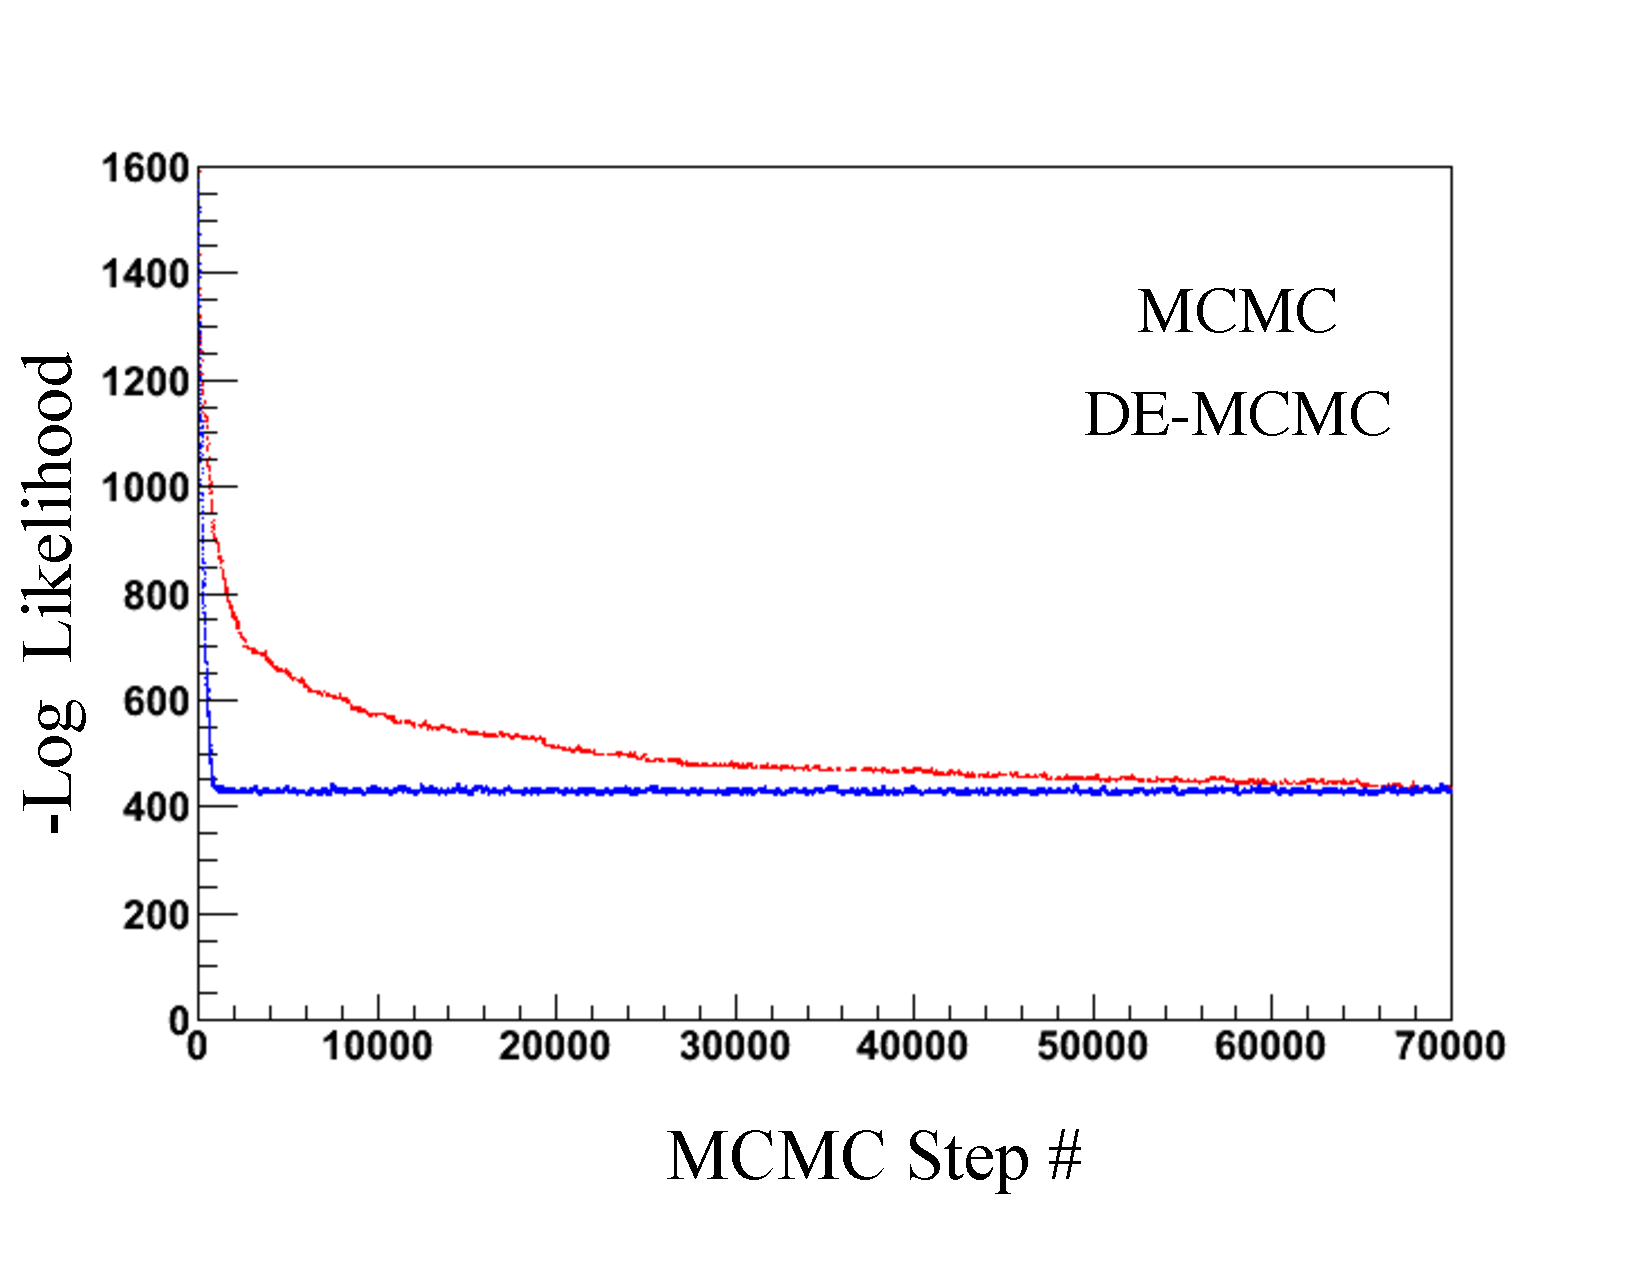
\includegraphics[width=0.5\textwidth]{plt_burnin}
\end{center}
\caption{Comparison of the burn-in period using an uncorrelated Gaussian
proposal fuction (red) and a proposal function that takes into account
parameter correlations using the DE-MCMC method (blue).  Both chains have been
tuned achieve an accpetance rate of $0.25\%$.}
\label{fig:burnin}
\end{figure}






